\documentclass{beamer}
\usetheme{metropolis}
\usepackage{appendixnumberbeamer}
\usepackage{subfigure}
\usepackage{booktabs}
\usepackage[scale=2]{ccicons}
\usepackage{pgfplots}
\usepackage{xspace}
\usepackage{graphicx}
\usepackage{listings}
\usepackage[english]{babel}
\usepackage{amsmath, amsfonts, epsfig, xspace}
\usepackage{algorithm,algorithmic}
\usepackage{multimedia}
\usepackage[T1]{fontenc}
\usepackage{roboto} 
\usepackage{epstopdf}
\usepackage{caption}
\epstopdfDeclareGraphicsRule{.gif}{png}{.png}{convert gif:#1 png:\OutputFile}
\AppendGraphicsExtensions{.gif}
%\usetheme{lankton-keynote}

\captionsetup{labelformat=empty}

\author{John Berlin}

\subtitle{
\normalsize{The Deep Web: Surfacing Hidden Value} \\  \footnotesize{Michael K. Bergman},  2001, Journal of Electronic Publishing\\ 
\normalsize{Searching for Hidden-Web Databases} \\ \footnotesize{Luciano Barbosa \& Juliana Freire}, 2005, Proceedings of WebDB
}

\title{Presentation 1}
\institute{Old Dominion University \\ Introduction to Information Retrieval \\ CS734/834   }


\begin{document}


\maketitle

\begin{frame}{Table of contents}
  \setbeamertemplate{section in toc}[sections numbered]
  \tableofcontents[hideallsubsections]
\end{frame}



\section{Introduction}
\subsection{What is the Deep Web?}

\begin{frame}[fragile]{What is the Deep Web?}
	%\onslide<1->{
	\begin{block}{Content not indexed (\alert{crawled}) by search engines}
	%\onslide<2->{
	This content is characterized as \emph{dynamic} and is generally \\
	generated as the result of a specific query
	%}
  \end{block}
  %}
   %\onslide<3->{
   \begin{columns}[T,onlytextwidth]
    \column{0.5\textwidth}
		\begin{block}{Where does the dynamic content come from?}
			\begin{itemize}
    %			\onslide<4->{
     			  \item Databases
    %			}
   	%			\onslide<5->{ 
   				 \item Forms
   	%			 }
  			\end{itemize}
  		\end{block}
	\column{0.5\textwidth}
  		\begin{figure}
			\includegraphics[scale=0.3]{invisible-web.gif}
		\end{figure}
  \end{columns}
  %}
\end{frame}

\section{The Deep Web: Surfacing Hidden Value}
\subsection{Contribution}
\begin{frame}{Bergman's Contribution}
\begin{block}{}
			\begin{itemize}
    %			\onslide<1->{
     			  \item A quantification for the size of the deep Web
    %			}
   	%			\onslide<2->{ 
   				 \item A characterization of the deep Web's contentent
   	%			 }
   	\item Initial enumeration of the difficulties for retrieving deep web content 
  			\end{itemize}
\end{block}
\end{frame}
\subsection{Quantification of the deep web}
\begin{frame}[fragile]{Quantification of the deep web}
To quantify the deep web a pool of 53,220 urls was used \\  
 43,348 retrieved and 700 were randomly selected \\
$13.6\% \approx 100$ were found not to be search sites i.e. Google like
but provided a lower bounds size estimation by content overlap
\begin{figure}
			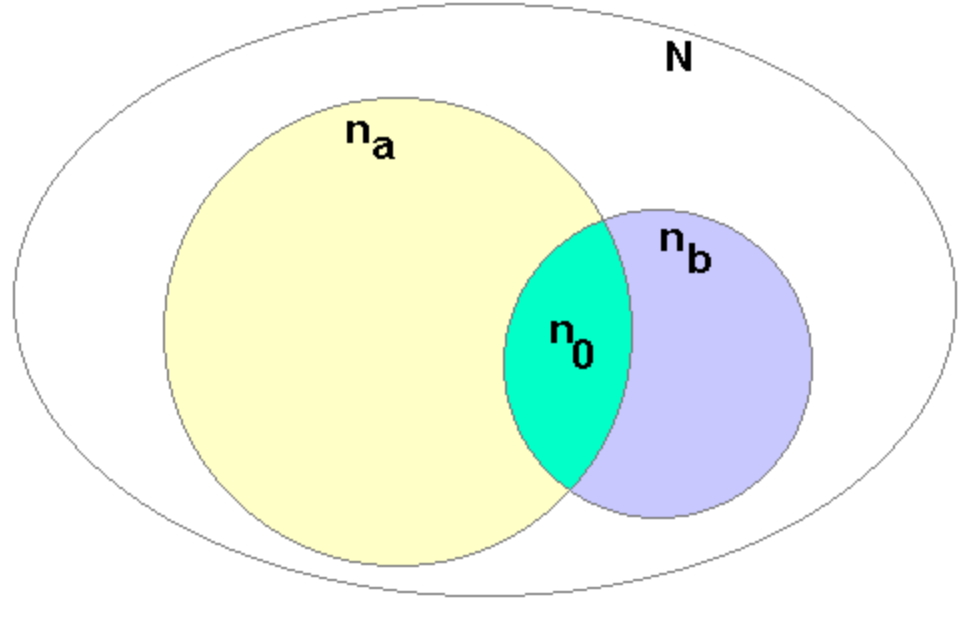
\includegraphics[height=3cm]{overlapAnalysis.png}
			\caption{Remember Lecture 1 WebSci \\ Figure 3 page 4}
	\end{figure}
\end{frame}
\begin{frame}[fragile]{Quantification of the deep web}
Another 100 random sites were chosen for content analysis \\
The html documents (records) per site was retrieved  \\
Mean size of 13.7KB, median 19.7KB  \\
Mean \#documents of 5.43 million, median 4.95 thousand \\
From this they estimated > 200,000 total deep web sites \\
For a total of 543 billion documents 
\begin{figure}

  \begin{minipage}[c]{0.3\textwidth}
   \caption{ \footnotesize{Inferred Distribution of Record Size} \\ Figure 4 page 8}
  \end{minipage}
			\begin{minipage}[c]{0.67\textwidth}
   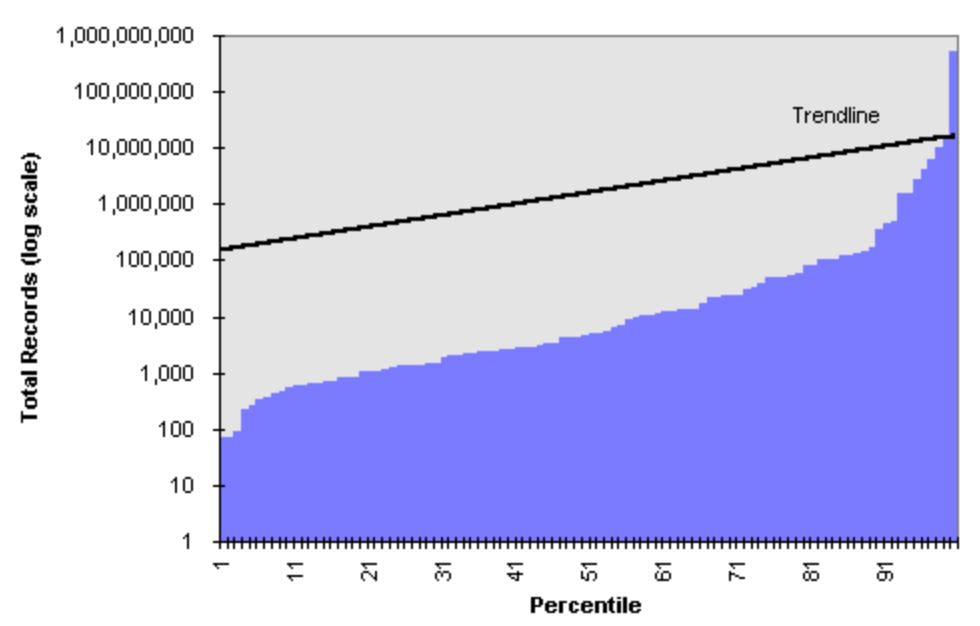
\includegraphics[height=4cm]{inferedDWRecSize.png}
  \end{minipage}
			
	\end{figure}
\end{frame}
\begin{frame}[fragile]{Quantification of the deep web}
Along with the documents the databases were retrieved \\
Mean size 74.4 MB with median of 169 KB \\
Estimated total database size of 7.44 petabytes \\
Compared to 18.7 terabytes of the surface web at the time \\
60 deep web sites had already known database size \\
totaling 750 terabytes \\
\begin{figure}
\begin{minipage}[c]{0.3\textwidth}
   \caption{\footnotesize{Inferred Distribution of Database  Size} \\ Figure 5 page 9}
  \end{minipage}
			\begin{minipage}[c]{0.67\textwidth}
  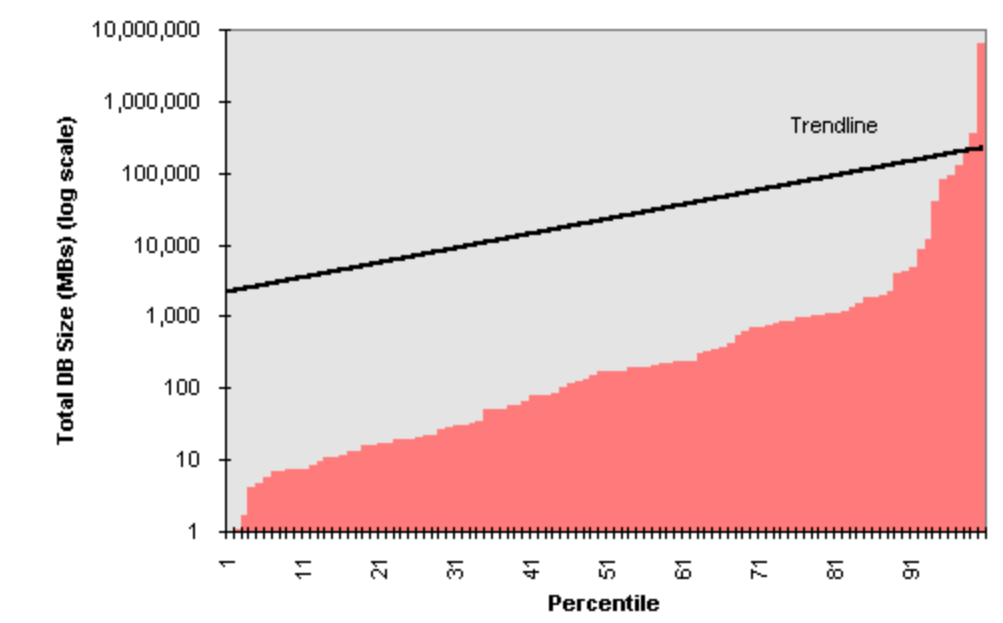
\includegraphics[height=4cm]{tdbSize.png}
  \end{minipage}
			
	\end{figure}

\end{frame}
\subsection{Characterization of the deep web}
\begin{frame}[fragile]{Characterization of the deep web}
\begin{columns}[T,onlytextwidth]
    \column{0.5\textwidth}
	Revisiting the initial 43,348 urls \\
	17,000 sites were selected \\ 
	For subject and content analysis \\
	It was found that they  \\
	contained an uniform subject \\
	distribution  \\
	Table 6, page 9 seen left shows these findings \\
	\column{0.5\textwidth}
  		\begin{figure}
			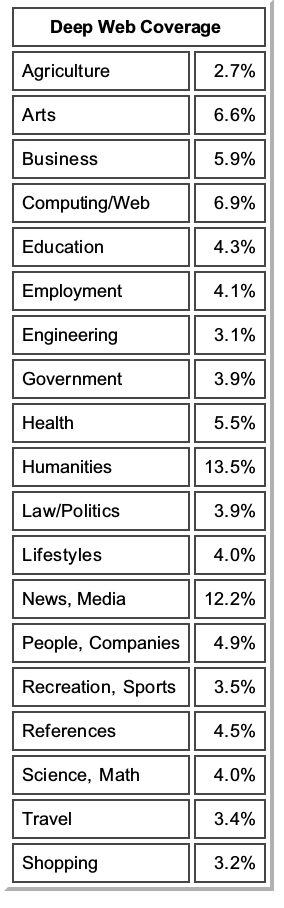
\includegraphics[height=8cm]{dwsubj.png}
		\end{figure}
  \end{columns}

\end{frame}
\begin{frame}[fragile]{Characterization of the deep web}
Topical databases, internal site documents and archived publications make up 80\% of all deep web sites\\
E-commerce along with auction and classified sites 10\% \\
Remaining sites 10\% 
\begin{figure}
			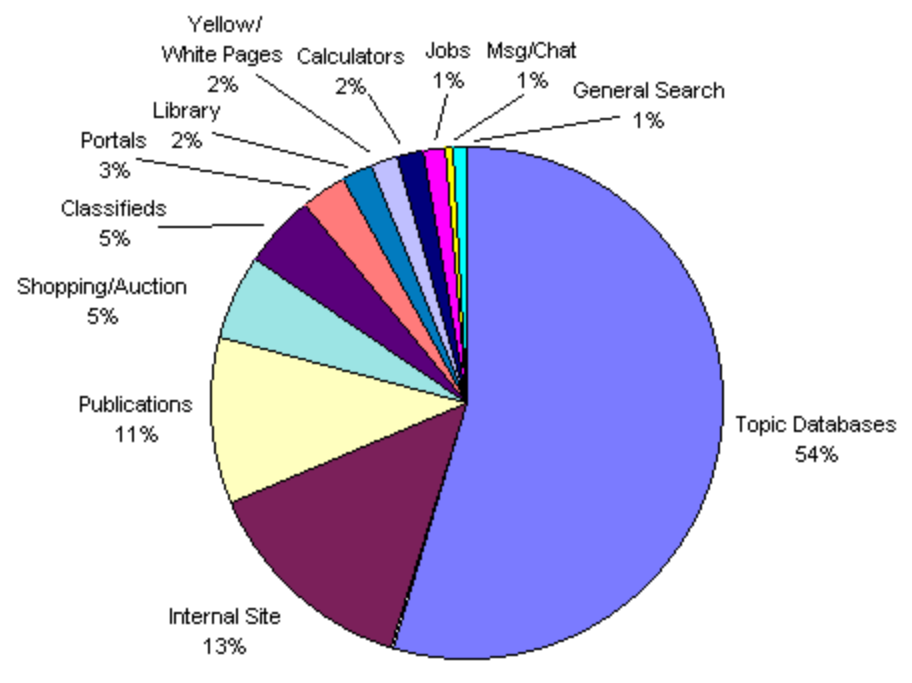
\includegraphics[width=6cm]{dwct.png}
			\caption{ Figure 6 page 10}
		\end{figure}
\end{frame}
\subsection{Difficulties in retrieving deep web content }
\begin{frame}[fragile]{Difficulties in retrieving deep web content }
\begin{block}{Database Content Retrieval Used In Study}
Directed queries are necessary 
using 21m terms, 430k unique \\
For each new database 430k queries are needed \\
To get all of their contents \\
An infeasible task at scale
\end{block}

\end{frame}
\begin{frame}[fragile]{Difficulties in retrieving deep web content }
\begin{block}{Search Engines Use Breath Crawls}
The query  \emph{URL:dmoz.org} was made to four major search engines \\
Dmoz or Open Directory had at the time subject structure of 248k categories \\
The search engines returned only a small percentage of expected results
\end{block}
\begin{figure}
			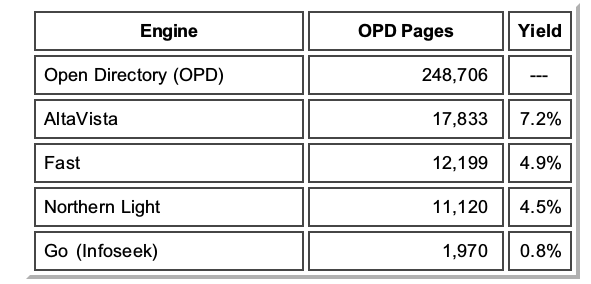
\includegraphics[width=6cm]{dwII.png}
			\caption{Table 7 page 10}
		\end{figure}
\end{frame}
\begin{frame}[fragile]{Difficulties in retrieving deep web content }
Leaving the question of how to effectively access the contents of the deep 
web databases and crawl sites in order to find links to the deeper content open
\end{frame}
\section{Searching for Hidden-Web Databases}
\subsection{Contribution}
\begin{frame}{ Barbosa \&  Freire's Contribution}
New Crawling Strategy to automatically discover hidden-web databases
\end{frame}

\begin{frame}{ Form-Focused Crawler}
\begin{block}{Depth Focused Crawling}
Avoid links that lead to off-topic regions \\
Back the crawler with a classifier to determine what is relevant \\
The classifier is trained on the pages belonging to topics in a taxonomy e.g. \emph{dmoz.org} \\
Links are then given to another classifier to select the most promising links in the selected page.
\end{block}
\end{frame} 
\begin{frame}{ Form-Focused Crawler}
\begin{block}{Crawler that understands form interfaces}
Deep web use forms as the front end to databases \\
Must know what forms are searchable or not e.g. logins \\
And be domain-independent \\
To do this the crawler uses a third classifier for forms
\end{block}
\begin{figure}
			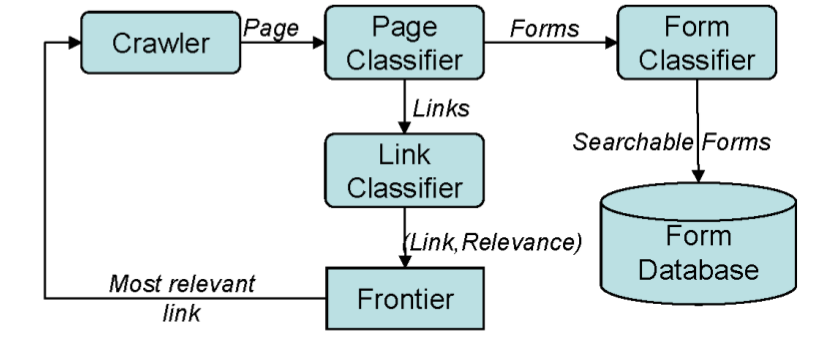
\includegraphics[width=6cm]{fca.png}
			\caption{\footnotesize{Form Crawler Architecture} \\ Figure 1 page 3}
		\end{figure}
\end{frame}
\subsection{Classifier Setup}
\begin{frame}{Classifier Setup}
\begin{block}{Link Classifier}
Forms are sparsely distributed \\
Selecting links with immediate benefit means you miss forms \\
This classifier identifies links that bring \emph{delayed benefit} \\
Or links that will \emph{eventually} lead to forms \\
In order to know what links will do that depends on training \\
\end{block}
\end{frame}
\begin{frame}{Classifier Setup}
\begin{block}{Link Classifier - Feature space by back crawling}
Approximation of the connectivity graph for a site \\
Using Google's ``link:'' searches conduct bread-first crawl \\
Starting with pages that have a searchable form \emph{level 1} \\
Find links that point to the form level+1 \\
Count features in url string and document text \\
\end{block}
\begin{figure}
			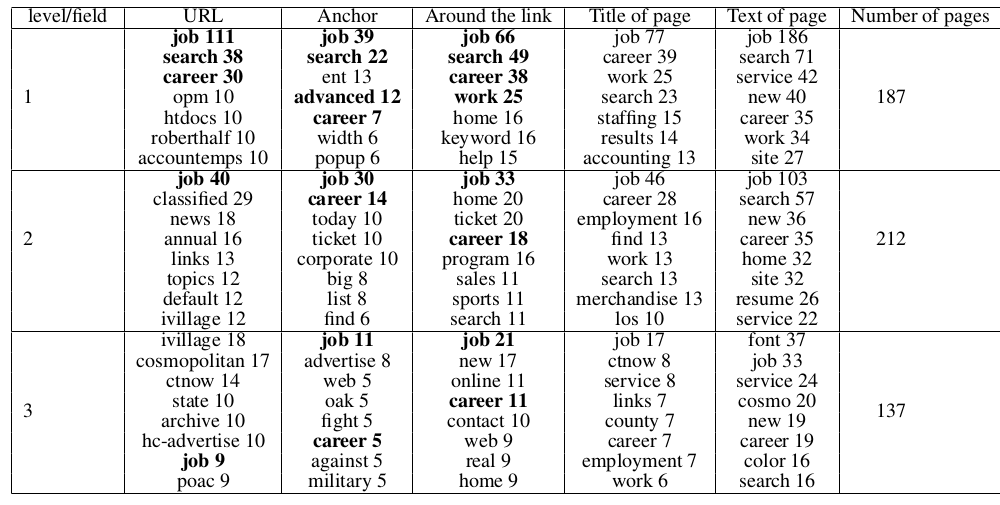
\includegraphics[scale=0.23]{lfs.png}
			\caption{\footnotesize{Feature Space For Job Domain} ,Table 1 page 4}
		\end{figure}
\end{frame}
\begin{frame}{Classifier Setup}
\begin{block}{Page Classifier}
Uses the Rainbow classifier, na{\"i}ve Bayes \\
Trained on pages from \emph{dmoz.org} \\
Gives a score if the page belongs to the focus topic \\
\end{block}
\begin{block}{Form Classifier}
Decision Tree classifier (C4.5) to determine searchability \\
Trained by finding number of tags, input fields, size of text and submission method (post or get) 
\end{block}
\begin{figure}
			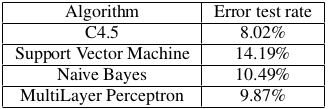
\includegraphics[scale=0.4]{cer.png}
			\caption{\footnotesize{Test error rates for different learning algorithms} \\ Table 2 page 4}
		\end{figure}
\end{frame}
\subsection{Crawl Strategy}
\begin{frame}{Crawl Strategy}
\begin{block}{Frontier Generation}
$N$ queues determined by the number of levels used by the link classifier \\
Prioritize links closer to target page \\
Queues ordered by likelihood of belonging to a level \\
\end{block}
\begin{block}{Stopping Criteria}
When a predetermined number of forms  has been retrieved \\
Estimated 4.2 query interfaces (form) on any given deep web site \\
Visited maximum number pages on a site \\ 
\end{block}
\end{frame}
\subsection{Crawler Performance}
\begin{frame}[fragile]{Crawler Performance}
\begin{columns}[T,onlytextwidth]
    \column{0.5\textwidth}
	\begin{figure*}
\captionsetup[subfigure]{labelformat=empty}
\subfigure{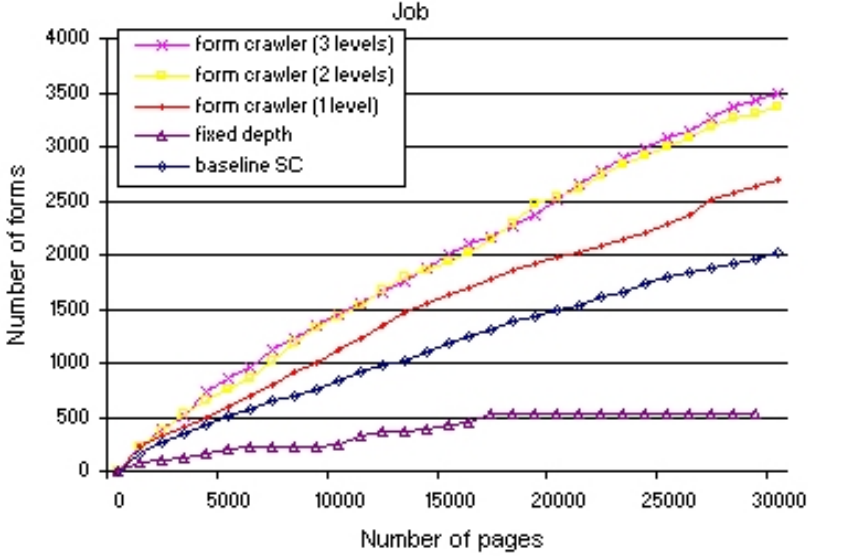
\includegraphics[width=\linewidth]{jobDomainCP.png}} 
\subfigure{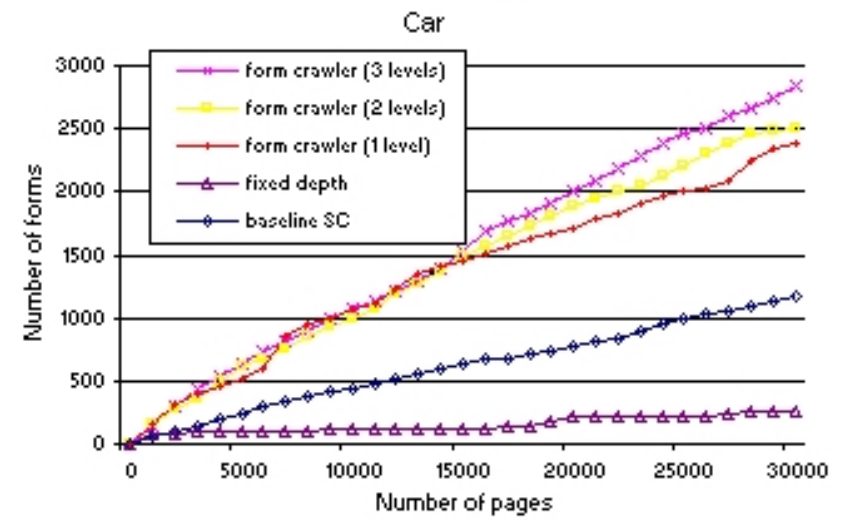
\includegraphics[width=\linewidth]{carDomainCP.png}} 
\end{figure*}
	\column{0.5\textwidth}
  		\begin{figure}
		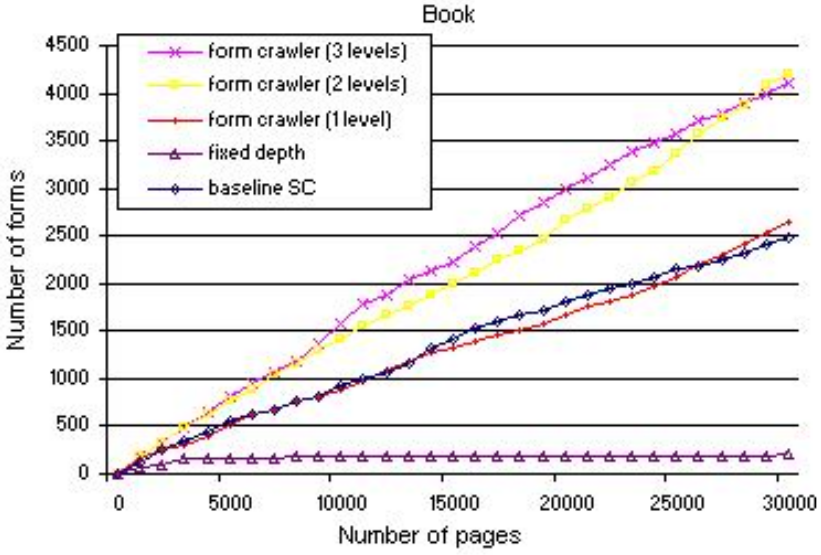
\includegraphics[width=\linewidth]{bookDomainCP.png}
		\caption{Figure 2 page 5}
		\end{figure}
       \ \  Using 3 vs 1 level configuration \\ \ \ Gain improvements of \\ \ \ 20\% to 30\% \\
  \end{columns}
\end{frame}
\section{Conclusion}
\begin{frame}[fragile]{Conclusion}
\begin{block}{The Deep Web: Surfacing Hidden Value}
Bergman provided a measurement for the deep web \\
Showed its content is highly relevant to surface web searches \\
Enumerated on the difficulties of crawling and extracting the content
\end{block}
\begin{block}{Searching for Hidden-Web Databases}
Barbosa \& Juliana built a crawler to address the issue of  \\
database discovery that Bergman highlighted \\
\end{block}
\end{frame}
\end{document}
